
\newcommand{\erdosrenyi}{Erd\"{o}s-R\'{e}nyi }

\subsection{Applications: Random Graphs}

At the intersection of graph theory and probability lies the Erd\"{o}s-R\'{e}nyi model. It is one of the simplest random graphs. The model has $n$ vertices, and the vertices are connected with some probability $p$; we denote such a graph as $G(n, p).$ \\ 

As a brief analysis on the \erdosrenyi model, let us study the expected number of edges per vertex. For every vertex, there are $(n-1)$ possible edges. However, since there is a fixed probability, $p$, of having a connection between verticies, the number of edges per vertex may be modeled as a binomial random variable $D$. Therefore, using the expectation of a binomial random variable, the expected number of edges per vertex is $d = E[D] = (n-1)p$. \\ 

\begin{tcolorbox}
\begin{definition}[Dense Graph]
A random graph $G(n, p)$ is said to be relatively \textit{dense} if the expected degree of each vertex is $E[D]= d \gtrsim \log{n}. $
\end{definition}
\end{tcolorbox}


% =======================================
% Proposition: Regularity of Dense Graphs
% =======================================
\begin{tcolorbox}
\begin{proposition}[Regularity of Dense Graphs]
Consider a random graph $G\sim G(n, p)$ with the expected degree $E[D] = d: d\geq C\log{n}$, where $C$ is some fixed constant. It follows that there is a probability $1-\varepsilon$ that all vertices within $G$ have degrees between $(1-\varepsilon) d$ and $(1+\varepsilon) d$. 
\end{proposition}
\end{tcolorbox}

% =====
% PROOF
% =====
\begin{proof}
To begin, we will work with an individual vertex $i$ within the graph $G$. Recall that we have already noted that the number of edges per vertex $D_i \sim binomial(n-1, p)$. Equivalently, we may say that the number of edges per vertex is represented by $D_i \sim \sum_{i=1}^{n-1} X_i$ where $X_i \sim Bernoulli(p).$ Since we have shown that we are working with sums of Bernoulli random variables, we may use the Chernoff bound.  \\ 

Using the small-deviations representation of the Chernoff bound in Equation $\ref{eq:chernoff2}$, we obtain 
$$ P\left( |D_i - d| \geq \varepsilon d \right) \leq 2e^{-cd}. $$
Now, when we consider all vertices in the graph, we find that 
    \begin{align*}
    P\left( \exists i\leq n: |D_i - d| \geq \varepsilon d \right) &\leq \sum_{i=1}^{n}P\left( |D_i - d| \geq \varepsilon d\right) && \text{Union bound ???} \\ 
    &\leq n \cdot 2e^{-cd} && \text{Chernoff's inequality for each vertex} \\ 
    &= \frac{2n}{e^{cd}}  \\ 
    &\leq \varepsilon &&\text{for large enough $c$} 
    \end{align*}
With our goal now to take the complimentary event, we have 
    \begin{align*}
    P\left( \exists i\leq n: |D_i - d| \geq \varepsilon d \right) &\leq \varepsilon &&\text{from previous} \\ 
    -P\left( \exists i\leq n: |D_i - d| \geq \varepsilon d \right) &\geq -\varepsilon &&\text{multiply both sides by $-1$} \\ 
    1-P\left( \exists i\leq n: |D_i - d| \geq \varepsilon d \right) &\geq 1-\varepsilon &&\text{add $1$ to both sides} \\ 
    P\left( \forall i \leq n: |D_i - d| < \varepsilon d \right) &\geq 1-\varepsilon &&\text{definition of complement} 
    \end{align*}
    That is, for arbitrary probability, we can create bounds for the number of degrees per vertex in the random graph.  
\end{proof}


\begin{tcolorbox}
    \begin{definition}[Big O Notation]
    $f(x) = O(g(x)) \iff \lim_{x\to\infty} f(x)/g(x) = C$
    \end{definition}
%
    \begin{definition}[o Notation]
    $f(x) = o(g(x)) \iff \lim_{x\to\infty} f(x)/g(x) = 0$ 
    \end{definition}
\end{tcolorbox}


\begin{figure}[H]
        \centering
        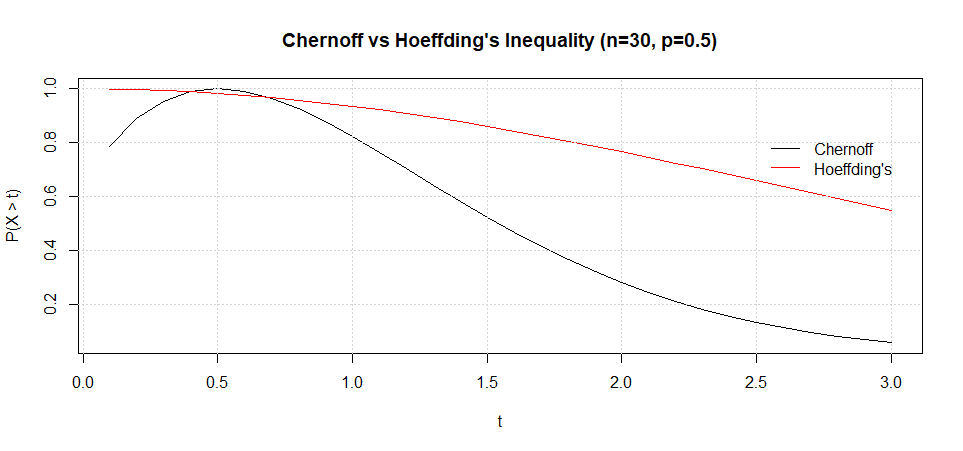
\includegraphics[scale=0.6]{Chernoff_Vs_Hoeffding}
        \caption{Hoeffding's inequality is not as sensitive as Chernoff's bound for means. }
\end{figure}